\documentclass[a4paper,10pt]{article}
\usepackage[T2A]{fontenc}
\usepackage[utf8x]{inputenc}
\usepackage{ucs}
\usepackage{cmap}
\usepackage[english,russian]{babel}
\usepackage{amsmath}
\usepackage{color,graphicx}
\usepackage{indentfirst}
\usepackage{ucs} 
\usepackage[utf8x]{inputenc}
\usepackage{caption}
\usepackage{placeins}
\usepackage{amssymb}

\title{Обзор спайковых сетей}
\author{Чернышев Алексей}
\setlength{\parindent}{1cm}
\def\la{\left\langle\rule{0pt}{3em}}
\def\ra{\right\rangle}
\newcommand{\HRule}{\rule{\linewidth}{0.5mm}}



\begin{document}
\begin{titlepage}
\begin{center}
% Title
\HRule \\[0.4cm]
{ \huge \bfseries Cпайковые нейронные сети \\[0.4cm] }

\HRule \\[1.5cm]
% Author and supervisor
\begin{minipage}{0.4\textwidth}
\begin{flushleft} \large
\emph{Автор:}\\
асп. Чернышев Алексей
\end{flushleft}
\end{minipage}
\begin{minipage}{0.4\textwidth}
\begin{flushright} \large
\emph{Научный руководитель:} \\
д.ф.-т.н. Карпенко А.П.
\end{flushright}
\end{minipage}

\vfill

% Bottom of the page
{\large Август 2014}

\end{center}
\end{titlepage}


\tableofcontents
\clearpage
\section{Введение}
\indent Нейронные сети, как попытка воссоздать процессы интеллектуальной информационной обработки, происходящие в коре головного мозга, являются предметом исследования учёных больше полувека. Наработанные знания в этой сфере образовали такую область научных исследований, как нейроинформатика и теоретическая нейронаука.\\
\indent Первый взрыв интереса к нейронным сетям был подпитан гипотезой об устройстве мыслительного процесса аналогично машине фон-Неймана, когда каждый нейрон представлялся логической функцией из элементарной логики, и соединение таких нейронов в сети формировало сложную иерархическую логическую функцию. Именно в это время получили своё начало модели подобные нейрону МакКалока-Питтса (1943), которые являются до сих пор наиболее популярным решением, предлагаемое теорией нейронных сетей.\\
\indent Начиная с 1943, исследования процессов мышления и нейронов, как биологических элементов, значительно продвинулись, в особенности с появлением функциональной томографии и микроэлектродов в последние 20 лет. Таким образом, сегодня нейроинформатика находится под влиянием переосмысления новых открытых качеств нейронов\cite{BohteReview}, как информационных вычислительных элементов.\\
\indent Спайковые нейронные сети являются той подобластью нейронного моделирования, которая концентрирует своё внимание на биологических деталях с целью поиска новых перспектив в изучении нейронных процессов.\\
\indent В обзоре рассматриваются спайковые модели нейронов, нейронных сетей и алгоритмов их обучения, которые в той или иной степени приближены к биологическому правдоподобию. Рассматриваются примеры использования таких сетей как целью теоретических исследований, так и с целью прикладных применений.\\
\section{Биологическая основа нейронов}
\indent Человеческий мозг содержит в себе огромное количество соединенных между собой нейронов (нервных клеток), которые стали предметом интереса во многих областях, таких как нейрофизиология, теоретическая нейронаука, искусственный интеллект.\\
\indent Нейрон по своему строению довольно схож с другими клетками: тело нейрона окружено плазматической мембраной, внутри которой находятся ядро, цитоплазма и другие составляющие клетки. Однако нейрон несет в себе особую функцию: нейрон выполняет приём сигналов от других нейронов, преобразует и передает их на вход других нейронов или клеток. Сигнал представляет собой импульсы нервной активности, имеющих электрохимическую природу.\\
\indent Нейроны крайне разнообразны по форме и нюансам функционирования, хотя существует возможность вывести наиболее типичную форму нейрона. На рис. \ref{bio_pic} отображена схема биологического нейрона. \\
\begin{figure}[ht]
\centering
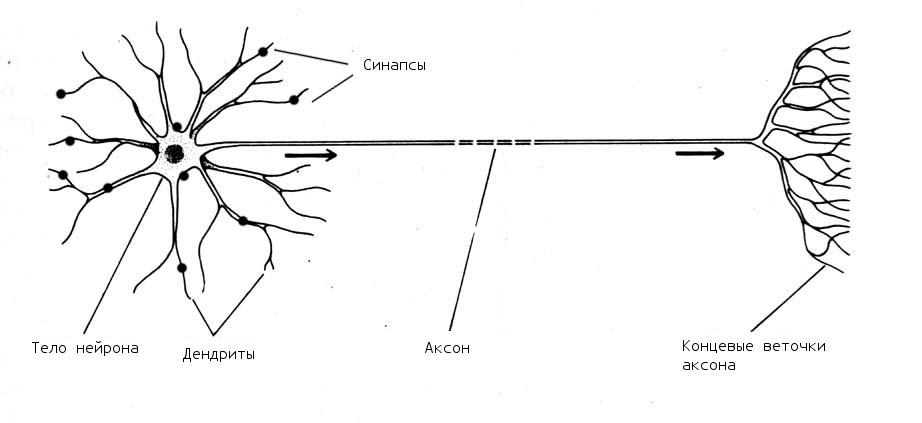
\includegraphics[width=1\linewidth]{bio_neuron.jpg}
\caption{Биологический нейрон}
\label{bio_pic}
\end{figure}
\indent Прием нервных импульсов от других нейронов происходит посредством дендритов, на которых расположены синапсы -- точки соединения нейронов между собой. Дендриты проводят входные импульсы с синапсов, доставляя их клетке нейрона, и специфичным образом возбуждая клеточную мембрану.\\
\indent Электрохимические процессы внутри клетки делают нейрон в той или иной мере чувствительным к возбуждениям мембраны, и когда возбуждение достигает определенного порога, потенциал на мембране в течение короткого времени (около 2 мс) осуществляет резкий скачок вверх, порождая короткий импульс, называемый спайком. Аксон является проводником таких импульсов к другим клеткам. После выработки спайка нейрон переживает т.н. рефракторный период, в течение которого чувствительность мембраны к возбуждениям резко спадает.\\
\indent Синапс, при более подробном взгляде, представляет собой не менее сложный механизм, чем сам нейрон. Типичный синапс, рассматривается как контакт между аксоном одного нейрона, называемого пресинаптическим, и дендритом другого, постсинаптического нейрона. На стороне аксона находится пузырек наполненный нейромедиаторами, а на стороне дендрита мембрана чувствительная к ним. При возбуждении аксона нейромедиаторы синапса начинают высвобождаться в пространство между пузырьком и мембраной -- синаптическую щель (10-50 нм). Достигнув постсинаптической мембраны нейромедиаторы могут быть ``схвачены'' чувствительными белками, которые находятся на ней, вызывая тем самым возбуждение мембраны. Следствием такой структуры является одностороннее проведение нервного импульса. Количество высвобожденного и принятого нейромедиатора варьируется, и ``натренированный'' синапс, проводит гораздо большее количество импульса за счёт большего количества нейромедиаторов в синаптическом пузырьке и рецепторов на постсинаптической мембране. В нейроинформатике обычно пренебрегают такими тонкими деталями и вводят ``веc'' синапса, который характеризует насколько эффективно синапс может проводить импульсы. Хотя существуют и другие виды синаптической передачи импульса, механизм описанный выше наиболее часто встречается в процессах формировании памяти.\\
\indent Ещё один феномен, касающийся нюансов функционирования биологического нейрона -- сенсорная адаптация\cite{Phizi}. Нейрон при получении импульсов с одной и той же характеристикой, как правило, начинает ``привыкать'' и приспосабливаться, чтобы тратить меньше энергии при интеграции этого сигнала. Как следствие, интенсивность его ответа угасает. В области теоретической нейронауки этот феномен довольно пристально исследуется и существуют выводы об оптимальности такого поведения с точки зрения оптимизации информации, переданной нейроном \cite{Adapt,TripleAdapt}.

\subsection{Модель Ходжкина-Хаксли}
	В 1952 году Алан Ллойд Ходжкин и Эндрю Хаксли разработали первую, наиболее подробную на тот момент математическую модель нейрона. Модель была построена на основе динамики генерации и передачи нервного сигнала в гигантском аксоне кальмара.\\
	\indent Данную модель сложно применить к решению реальных задач нейроинформатики, так как её симуляция ресурсоёмка -- около 1200 операций с плавающей точкой для моделирования одной миллисекунды\cite{BohteReview}. Однако эта модель играет важную научную и историческую роль в нейронауке.\\
	\indent Общая динамика потенциала нейрона описывается плавным затуханием значения потенциала $u_{m}(t)$ на, со скоростью, которая характеризуется ёмкостью мембраны $C_{m}$
	\begin{equation}\label{eq:hh}
	C_{m}\frac{du_{m}}{dt}+I_{ion}(t)=I_{ext}(t).
	\end{equation}	 
	Здесь $I_{ion}(t)$ - сумма ионных токов внутри клетки, $I_{ext}(t)$ - ток снаружи клетки.\\
	\indent Сложность уравнения \eqref{eq:hh}	 таится в моделировании ионных токов для каждого типа ионов. В модели Ходжкина-Хаксли динамика ионных токов характеризуется наличием т.н. ионных каналов, открытие или закрытие которых влияет на общую динамику напряжения на мембране. В исходной модели Ходжкина-Хаксли фигурируют два вида ионов $Na^{+}$ и $K^{-}$. Ионный поток $Na^{+}$ описывается тремя каналами, вероятность открытия которых равна $p_{m}$, и одним каналом с вероятностью открытия $p_{h}$. Ионный поток $K^{-}$ описывается четырьмя каналами с вероятностью открытия $p_{n}$\cite{Genesis}.\\ 
	\indent Динамика вероятности открытия-закрытия каналов, выражается дифференциальным уравнением первого порядка
	\begin{equation}\label{eq:hh_pch}
	\frac{dp_{i}}{dt} = \alpha_{i}(u_{m}(t))(1-p_{i}(t)) - \beta_{i}(u_{m}(t))p_{i}(t), \mbox{ для } i = m, h, n,
	\end{equation}	 
	где $\alpha_{i}(u_{m}(t)), \beta_{i}(u_{m}(t))$ константы, зависящие от потенциала на мембране, которые характеризуют скорость закрытия и открытия канала соответственно. Временной промежуток, спустя который вероятность достигает равновесия, описывается константой
	\begin{equation}\label{eq:hh_t}
	\tau_{i}=\frac{1}{\alpha_{i}(u_{m}(t))+\beta_{i}(u_{m}(t))}.	
	\end{equation}
	\indent Таким образом, динамику ионных токов для модели Ходжкина-Хаксли, можно описать уравнением
	\begin{align}\label{eq:hh_ion}
	I_{ion}(t) &= \begin{aligned}[t]
	&\bar{g}_{Na}\;p_{m}^{\;3}(t)\;p_{h}(t)\;(u_{m}(t)-E_{Na}) +	\\
	+\;&\bar{g}_{K}\;p_{n}^{\;4}(t)\;(u_{m}(t)-E_{K})+\bar{g}_{L}(u_{m}(t)-E_{L}),	\\
	\end{aligned}	
	\end{align}
	где $p_{m}(t), p_{h}(t), p_{n}(t)$ -- вероятности открытия каналов, описываются уравнением динамики \eqref{eq:hh_pch}, которые включают соответствующие константы. Смысл и значения констант из формулы \eqref{eq:hh_ion} можно найти в оригинальной работе\cite{HH}.\\
	\indent Несмотря на то что применение такой модели в задачах машинного обучения затруднительно, эта модель хорошо отражает всю сложность динамики биологического нейрона.

\section{Модели нейронов}
\subsection{Классические ИНС}
\subsubsection{Нейрон МакКалока-Питтса}
   Первая модель нейрона, положившая начало нейроинформатике -- модель МакКаллока-Питтса. Модель заложила фундамент теории нейронных сетей, и исследования новых свойств этой модели не прекращаются по сей день.\\
   \indent Ключевой особенностью данной модели является то, что нейрон представляется, как взвешенный сумматор входных характерных признаков $\boldsymbol{x}=(x_{1},x_{2},...,x_{n}) \in \mathbb{R}^n$. Обработка нейроном входов происходит пропусканием полученной суммы через нелинейную функцию $\phi(\boldsymbol{x})$, называемую функцией активации:\\
   \begin{equation}\label{eq:sum_mp}
   y(\boldsymbol{x}) = \phi(\sum_{j=1}^{n}w_{j}x_{j}).
   \end{equation}
\indent Здесь $\boldsymbol{w}=(w_{1}, w_{2},...,w_{n})$ вектор весов сумматора (синапсов нейрона), $y(\boldsymbol{x})$ - скалярная величина -- результат обработки нейроном вектора $\boldsymbol{x}$.\\	
	\indent В качестве нелинейной функции $\phi(x)$, наиболее популярным выбором является сигмоидальная функция\cite{Zaencev1999}. Эта функция удобна своей непрерывностью и гладкостью, и позволяет ограничить выход нейрона  отрезком значений $[0,1]$. Такой выход можно интерпретировать как уровень активации нейрона, что имеет свои, пусть и отдаленные, биологические основания. \\
   \indent Несмотря на ошеломляющий успех и широкое применение данной модели  и производных моделей в прикладных задачах, с биологической точки зрения такие нейроны, только отдаленно напоминают то, как работают настоящие нейроны в коре головного мозга.\\
   \indent Важным отличием такого нейрона от биологического является то, что модель не имеет внутреннего состояния и не может быть представлена в виде динамической системы\cite{Zaencev1999}. Это свойство серьезно ограничивает круг задач в которых можно было бы применить нейронные сети на основе модели МакКалока-Питтса. 
\subsubsection{Радиальный нейрон}
\indent Когда как нейрон МакКалока-Питтса имеет такую функцию активации которая позволяет нейрону иметь ненулевое значение активации на всем  диапазоне входных данных, радиальный нейрон имеет в своей основе функцию активации с локальным центром, и совсем не факт, что один такой нейрон охватит весь входной диапазон. Поэтому чаще всего рассматривают популяцию радиальных нейронов, или иначе говоря, радиальные сети.\\ 
\indent Радиальные сети исторически возникли на базе сочетания теории приближений и нейронных сетей. Элементарного элементом для построения сетей из радиальных нейронов служит аппроксимирующая функция-нейрон, линейная комбинация результатов активации $N$ нейронов выражается значением функции $y(\boldsymbol{x}), x\in \mathbb{R}^n$
   \begin{equation*}\label{eq:rbf}
   y(\boldsymbol{x}) = \sum_{i=1}^{N}w_{i}\phi(|\boldsymbol{x}-C_{i}|),
   \end{equation*}
где $w_{i}$ - вес $i$-ого нейрона, модулирующий его вклад в вычисление, $C_{i}$ - центр функции активации, который задаёт область чувствительности для $i$-ого нейрона.\\
\indent Несмотря на то, что радиальный нейрон также как и нейрон МакКалока-Питтса не имеет внутреннего состояния, локальность, которая является ключевой особенностью радиальный сетей, является биологически оправданным фактором, который мождно найти в ряде нейронных систем.\\

\subsection{Спайковые модели}   
\subsubsection{Пороговый интегратор}

\indent Пороговый интегратор (англ. Integrate-and-fire) имеет большую историю. Ещё в 1907 году 	французский физиолог Луи Лапик экспериментируя с лягушками, описал модель возбуждения нервных клеток используя RC-цепь\cite{Lapicque}, которая лежит в основе порогового интегратора. За свою вековую историю модель благодаря своей простоте и, главное, биологической оправданности, получила много применений.\\
   \indent Пороговый интегратор представляет собой динамическую систему с одной переменной, довольно похожей на уравнение \eqref{eq:hh}, за тем исключением, что ионные токи не моделируются, а спайк генерируется нейроном при достижении заранее заданного порога:\\
   \begin{equation}\label{eq:iaf}
   \tau_{m}\frac{du}{dt} =-u(t)+R I(t).
   \end{equation}
При $u(t) \geq \vartheta$ потенциал мембраны сбрасывается, то есть принимается $u(t)=u_{r}$.
Здесь $\vartheta$ - порог напряжения; $\tau_{m}=RC$ временная константа мембраны ; $R$ и $C$ - сопротивление и ёмкость RC-цепи соответственно, $I(t)$ - ток, приложенный извне, $u_{r}$ - константа описывающая потенциал мембраны покоя нейрона.\\   
\indent Данная нейронная модель подходит для конструирования нейронных сетей: приложенный ток $I(t)$ можно рассматривать, как ток, получаемый нейроном через синапсы от других нейронов. Допустим, нейрон соединён с N входными спайковыми нейронами через синапсы с определенными весами. Тогда приложенный ток описывает равенство
\begin{equation}\label{eq:iaf_syn}
I(t) = \sum_{j=1}^{N} \sum_{t_{j}^{f}\in X_{j}} w_{j}\; \epsilon(t-t_{j}^{f}),
\end{equation}
где $\epsilon(t)$ - низкочастотный фильтр, который характеризует спайк на синапсе, $w_{j}$ - вес синапса, $t_{j}^{f}$ - время спайка на входном нейроне, $X_{j}$ - набор спайковых времён на синапсе. Фильтр $\epsilon(t)$ как правило выбирают виде затухающей экспоненты, такая функция хорошо описывает импульс переданный в процессе передачи нейромедиаторов.\\

\subsubsection{Модель Ижикевича}
\indent Данная модель является наиболее популярным компромиссом между вычислительной сложностью модели и её биоподобности. Модель описывается динамической системой с двумя переменными и квадратичной зависимостью. При хорошем подборе коэффициентов системы модель может воспроизводить большинство известных нейронных паттернов\cite{IzhSimpleModel}, включая, например, такие сложные как, высокочастотные спайки (fast spiking) или взрывной поток спайковых импульсов (bursting).\\
\indent Модель описывается системой уравнений
\begin{equation}\label{eq:izh}
\left\{  \begin{array}{c} \begin{aligned}
	\frac{du}{dt} &= 0,04u(t)^2+5u(t)+140-r(t), \nonumber \\
	\frac{dr}{dt} &= a(bu(t)-r(t)), \nonumber 
	\end{aligned}	
	\end{array} \right.
\end{equation}
где при $u(t) \geq \vartheta$ переменные сбрасываются:
\begin{equation}\label{eq:izh_reset}
\left\{  \begin{array}{c} \begin{aligned}
	u(t) &\leftarrow c \nonumber, \\
	r(t) &\leftarrow r(t)+d.
	\end{aligned}	
	\end{array} \right.
\end{equation}
Здесь приняты обозначения: $u(t), r(t)$ - переменные динамической системы; $a, b, c, d, \vartheta$ - константы. Переменная $u(t)$ отвечает за потенциал мембраны, $r(t)$ - переменная отвечающая за восстановление нейрона. Преодоления порога, описываемого константой $\vartheta$ и сброс переменных влечет за собой выработку нейроном спайка.\\
\indent Пониженная вычисляемая сложность делает эту модель наиболее подходящей для масштабных и правдоподобных симуляций головного мозга. Автором этой модели была проделана работа \cite{IzhTalam} по симуляции 3x3 см$^2$ таламо-кортикальной системы млекопитающего, включающей в себя $10^{11}$ нейронов и $10^{15}$ синапсов.
\subsubsection{Модель спайкового отклика}\label{sec:srm}
\indent Отдельным рядом стоит модель спайкового отклика (англ. Spike Response Model, SRM). В своём оригинальном виде модель повторяет динамику модели порогового интегратора и, по сути, является его приближенным решением.\\ 
\indent Генерация спайков происходит как и в пороговом интеграторе: при преодолении заданного порога, нейрон генерирует спайк. Однако, тогда как пороговый интегратор представляется в виде дифференциального уравнения, SRM определяет функция от времени и совокупность фильтров:
\begin{equation}\label{eq:srm}
u(t) = u_{rest} + \sum_{j=1}^N w_{j} \sum_{t^{f}_{j} \in X_{j}} \epsilon_{j}(t-t^{f}_{j}) + \sum_{t^{f}_{i}\in Y}\eta(t-t^{f}_{i}).
\end{equation}
Здесь $u_{rest}$ - константа описывающая потенциал покоя; второе слагаемое представляет из себя интеграцию спайков с синапсов. Cумма по $t^{f}_{j} \in X_{j}$ в этом выражении происходит по всем временам спайков $t^{f}_{j}$ на синапсе $j$ и $X_{j}$ представляет набор всех спайков на синапсе. Для каждого времени спайка при помощи низкочастного фильтра $\epsilon(\cdot)$ задаётся вклад данного спайка в потенциал на синапсе $j$ в текущий момент времени $t$. Полученный потенциал синапса, модулируемый его весом $w_{j}$, суммируется по всем синапсам нейрона. Третье слагаемое описывает суммацию всех спайков нейрона $Y$, пропущенных через фильтр $\eta(\cdot)$, функция которого описывает поведение нейрона после спайка. Такая функция позволяет спайкам нейрона в прошлом повлиять на текущее состояние мембраны $u(t)$. Как правило, этой функцией описывается состояние рефрактерности нейрона.\\
\indent Тот факт, что эта модель описывается функцией времени, позволяет напрямую выразить плотность вероятности спайков, пропустив напряжение на мембране через любую монотонно возрастающую функцию. Удобнее всего использовать экспоненциальный вид функции. Иногда эту функцию модифицируют так, чтобы вблизи определенного порогового значения мембраны вероятность генерации спайка резко возрастала. Вывод плотности вероятности позволяет описать процесс генерации спайка негомогенным пуассоновским процессом, что открывает широкие возможности для теоретического исследования спайкового нейрона.\\
\indent Добавление новых динамических свойств в SRM реализуется добавлением соотвествующих фильтров в уравнение \eqref{eq:srm} либо модификацией функции плотности вероятности\cite{TripleAdapt,AdaptThesis}. 

\section{Обучение нейронных сетей}
\subsection{Нейронные сети}
\indent Переход от изучения моделей нейронов к изучению их популяций естесственен -- известно, что биологические нейроны соединяются в сети и, тем самым, создают сложную распределённую модель обработки стимула. Однако для того чтобы сделать этот переход необходимо решить ряд вопросов относительно структуры модели:
\begin{itemize}
\item количество слоёв на которые делится популяция нейронов;
\item количество нейронов в каждой популяции;
\item паттерны соединения нейронов внутри слоя и между слоёв.
\end{itemize}
\indent Количество слоёв и нейронов, как правило зависит от поставленной задачи -- размеры сети можно подобрать кросс-валидацией \cite{krogh1995neural}. Паттерны соединения нейронов между собой задача более сложная, ввиду б\'{о}льшего количества переменных. В зависимости от паттернов соединения слоёв между собой нейронные сети принято разделять:
\begin{itemize}
\item сети прямого распространения;
\item рекурсивные сети.
\end{itemize}
В сетях прямого распространения слои нейронов распологаются в определённом порядке так что, сигнал из первого слоя достигает второго слоя, и только его, второй слой, в свою очередь передаёт сигнал третьему и т.д., пока сигнал не достигнет последнего слоя. Обратной связи в таких сетях не предусмотрено. К сетям прямого распространения можно отнести классические нейронные сети МакКаллока-Питтса.\\
\indent Рекурсивные сети содержат слои нейронов в которых разрешены соединения между неронами и соединения между слоями, как в прямом, так и в обратном направлении. Такой вид сетей более биоподобен, нежели сети прямого распространения, и, как правило, являются естесственным для спайковых нейронных сетей.\\
\subsection{Обучение классических ИНС}
\indent Наиболее устоявшимся методом обучения нейронных сетей является метод обратного распространения ошибки. Нейрон Маккалока-Питтса, имея в основе дифференируемую на множестве вещественных чисел функцию активации, прекрасно подходит для оптимизации весов нейрона с целью задавания необходимого выходного сигнала.\\  
\indent Метод обратного распространения ошибки решает задачу оптимизации весов нейронов всей сети в зависимости от функции оценки, которая количественно отражает, то насколько выход сети решает поставленную задачу. В качестве примера возьмём квадрат отклонения выхода нейрона последнего слоя сети от целевого значения:
\begin{equation}
E = \frac{1}{2}(y_{t}-y)^2,
\end{equation} 
где $E$ - ошибка ИНС, $y_{t}$ - целевое значение выхода ИНС, $y$ - выход ИНС.\\
\indent Пусть для нейрона $j$ с $n$ синапсами выход равен
\begin{equation}
o_{j}=\phi (\xi_{j}) = \phi \left(\sum_{k=1}^{n}w_{kj}x_{k}\right),
\end{equation}
где функция активации $\phi(z)$ нелинейная и дифференцируема, например
\begin{equation}\label{eq:logist}
\phi(z)=\frac{1}{1+\exp^{-z}},
\end{equation}
Тогда взять частную производную функции оценки по весам можно выразить через цепочку производных
\begin{equation}\label{eq:bp_chains}
\frac{\partial E}{\partial w_{ij}} = \frac{\partial E}{\partial o_{j}} \frac{{\partial o_{j}}}{\partial \xi_j} \frac{\partial \xi_j}{\partial w_{ij}},
\end{equation}
где последний член \eqref{eq:bp_chains} правой стороны имеет вид
\begin{equation}
\frac{{\partial \xi_{j}}}{\partial w_{ij}} = \frac{\partial}{\partial w_{ij}} \left(\sum_{k=1}^{n}w_{kj}x_{k}\right) = x_{i}.
\end{equation}
Частная производная выхода нейрона $j$ по параметру $\xi_{j}$ представляет собой частную производную функции активации, например для логистической функции \eqref{eq:logist} получаем
\begin{equation}
\frac{{\partial o_{j}}}{\partial \xi_{j}} = \frac{\partial}{\partial \xi_{j}} \phi(\xi_{j}) = \phi(\xi_{j})(1-\phi(\xi_{j})).
\end{equation}
Первый множитель уравнения \eqref{eq:bp_chains} выражается просто в случае, если нейрон принадлежит последнему слою
\begin{equation}
\frac{\partial E}{\partial o_{j}} = \frac{\partial E}{\partial y} = \frac{\partial}{\partial o_{j}} \frac{1}{2} (y_{t}-y)^2 = y - y_{t}  .
\end{equation}
В случае когда нейрон $j$ принадлежит внутреннему слою вычисления немногим усложняются. Рассмотрим функцию $E$ как функцию от $m$ входов нейронов предшествующего слоя:
\begin{equation}\label{eq:bp_rec}
\frac{\partial E(o_{j})}{\partial o_{j}} = \frac{E(\xi_{1}, \xi_{2},...,\xi_{m})}{\partial o_{j}}.
\end{equation}
Если взять полную производную по параметру $o_{j}$, рекурсивное выражение \eqref{eq:bp_rec} получает вид
\begin{equation}
\frac{\partial E}{\partial o_{j}} = \sum_{l\in L}\left(\frac{\partial E}{\partial \xi_{l}} \frac{\partial \xi_{l}}{\partial o_{j}}\right).
\end{equation}
\indent Собирая все выкладки вместе получаем
\begin{equation}\label{eq:bp_update}
\frac{\partial E}{\partial w_{ij}} = \delta_{j} x_{i},
\end{equation}
где
\begin{equation}
\begin{split}
\delta_{j} &= \frac{\partial E}{\partial o_{j}} \frac{\partial o_{j}}{\partial \xi_{j}} = \\ &=\begin{cases} (o_{j}-y_{t}) \phi(\xi_{j})(1-\phi(\xi_{j})), & \mbox{если }j\mbox{ -- выходной нейрон,} \\ (\sum_{k}\delta_{j}w_{jk})\phi(\xi_{j})(1-\phi(\xi_{j})), & \mbox{если }j\mbox{ -- нейрон сети.} \end{cases}
\end{split}
\end{equation}
\indent Обновление весов можно осуществлять, вычитая из $w_{ij}$ значение \eqref{eq:bp_update}, помноженного на небольшой коэффициент обучения, осуществляя тем самым минимизацию функции ошибки методом градиентного спуска.

\subsection{Биоподобное обучение ИНС}
\indent Под биоподобными правилами обучения нейронных сетей, здесь понимаются такие правила, которые основаны на воссоздании не сколько процессов происходящих в синапсе, но такие правила, которые могут воспроизвести наиболее важные аспекты информационной обработки биологическими нейронами и синапсами.\\
\indent Искусственным нейронным сетям для обучения по правилу обратного распространения ошибки необходим набор эталонных ответов, для того чтобы воссоздать статистическую связь между характерными признаками и ответом сети. Такой подход долго критиковался за свою биологическую неправдоподобность\cite{Uossermen}. Обучение без учителя, как возможность нейронной сети самостоятельно находить закономерности во входных признаках, считается наиболее биологически оправданным. Также стоит отметить, что в ИНС, в контексте любого правила обучения без учителя, должно быть однозначно ясно какое именно статистическое свойство входных данных определяет нейронная сеть в процессе обучения.\\

\subsubsection{Классическое правило Хэбба}\label{sec:hebb}
\indent Вопрос о том, как настоящий синапс обучается, стоит до сих пор, хотя огромное количество деталей этого процесса было открыто за последние полвека. Канадский физиолог Дональд Хэбб, ещё в 1949 году без возможности на тот момент проверить гипотезу заявил:\\
\indent ``Когда аксон нейрона А достаточно близок к тому чтобы возбудить нейрон Б и неоднократно или постоянно участвует в его активности, некоторые процессы роста или метаболических изменений имеют место в первой или обоих клетках, так, что эффективность возбуждения клеткой А клетку Б возрастает''\cite{Hebb1949}.\\
\indent Сейчас, когда современные технологии позволяют более детально изучить вопрос, можно сказать, что заявляение Хэбба было недалеко от истины. Было поставлено большое число экспериментов (см. обзор \cite{BiPoo}) для выявления зависимости между изменением веса синапса (пластичность) и активностей синапса и нейрона, которые породили обилие, как феноменологических, так и теоретических моделей.\\
\indent На сегодняшний момент можно оценить всплески интересов к этой области и разделить их на две ``эпохи'':
\begin{itemize}
\item пластичность синапсов на основе усреднённой активности нейронов (80-ые - конец 90-ых годов);
\item пластичность синапсов на основе точных времён спайков (конец 90-ых годов - по настоящее время).
\end{itemize}

\indent Такой перекос обозначается появлением в конце 90-ых годов прорывных исследований на тему спайко-временной пластичности \cite{stdp1,stdp2,stdp3,stdp4}. Этот феномен показывает как вес биологического синапса изменяется в зависимости от временной разницы между спайками на синапсе и на нейроне, что открывает новое пространство для исследований, в т.ч. и для исследования гипотезы, что природа спайкового кода может иметь временную основу.\\

\subsubsection{Пластичность на основе усреднённой активности}\label{sec:hebb}
\indent Пластичность весов на основе корреляции пресинаптической и постсинаптической активности можно представить в виде
\begin{equation}
\Delta w_{i} = \eta x_{i}y,
\end{equation}
где $\eta$ -- небольшой коэффициент обучения; $\Delta w_{i}$ -- изменение веса синапса $i$; $x_{i}$ - усреднённая активности нейрона, соединённого через синапс $i$; $y$ усреднённая активность самого нейрона.\\
\indent Такой вариант правила изменения весов ведёт к выделению нейроном главных компонент \cite{anderson1963} во входных признаках, но он нестабилен -- при применении на практике, $\Delta w$ всегда имеет положительное или отрицательное значение, что ведет к бесконечному росту или уменьшению весов в сторону наиболее сильной главной компоненты. Хотя, стоит отметить, что с биологической точки зрения, это проблема не столь существенна, так как синаптическая эффективность имеет свои ограничения в виде конечного числа нейромедиаторов и рецепторов на постсинаптической мембране\cite{NeuralAndAdaptiveSystems}.\\
\indent Тем не менее, проблема нестабильности правила Хэбба, породила множество исследований возможных модификаций этого правила. Наиболее ярким из них является решение проблемы финским учёным Е. Ойя, который вывел правило изменение весов в виде
\begin{equation}
\Delta w_{i} = \eta y (x_{i} - yw_{i}).
\end{equation}
Здесь выражение $yw_{i}$ создаёт обратную связь, которая ограничивает рост веса. Ойя показал, что такое правило ведет к росту весов, который максимизирует математическое ожидание квадрата выхода нейрона $y$, что совпадает с направлением первой главной компоненты, для данных с нулевым средним значением.\\
\indent Впоследствии Т. Зангер разработал расширение правила Ойя на сеть с $m$ выходами, где каждый выход соответствует первым $m$ главным компонентам:
\begin{equation}
\Delta w_{ij} = \eta y_{j} (x_{i} - \sum_{k=1}^{m}y_{k}w_{ki}),
\end{equation}
что можно считать альтернативным и в некоторых случаях более удобным подходом к выделению главных компонент.
\subsubsection{Теория БКМ}
\indent Теория БКМ (англ. BCM theory), названа в честь учёных разработавших её: Э. Бйаненшток, Л. Купер и П. Монро (E. Bienenstock, L.Cooper и P.Munro). БКМ -- это физическая теория описывающая обучение в зрительной коре. Данная теория знаменита своими предсказаниями, которые неоднократно подтверждались экспериментами \cite{Cooper}.\\
\indent Теория пластичности синапсов предлагаемая теорией БКМ имеет в своей основе правило Хэбба, и, по сути, является ещё одной модифицикацией, которая решает проблему стабильности классического правила Хэбба.\\
\indent Особенность пластичности синапсов в теории БКМ состоит в наличии т.н. плавающего порога $\theta_{M}$, который разделяет два режима пластичности: долговременная потенциация (Long-Term Potentiation, LTP); долговременная депрессия (Long-Term Depression, LTD). Таким образом, если активность нейрона $y<\theta_{M}$, то функция изменения весов $\Delta w<0$; если $y>\theta_{M}$, то $\Delta w>0$ и нейрон испытывает положительное изменение весов (рис. \ref{bcm_pic}).
\begin{figure}[ht]
\centering
\captionsetup{justification=centering,margin=1cm}
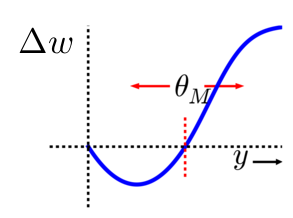
\includegraphics[width=60mm,scale=0.2]{bcm.png}
\caption{Плавающий порог БКМ правила}
\label{bcm_pic}
\end{figure}
\FloatBarrier
\indent Динамику весов нейрона, который описывает теория БКМ, можно выразить уравнением
\begin{equation}
\Delta w_{i} = y\,(y - \theta_{M})x_{i}\phi'(y)
\end{equation}
где $y$ - выход нейрона, который является линейной комбинацией входных сигналов с синапсов, пропущенной через нейлинейную функцию:
\begin{equation}
y = \phi(\sum_{j=1}^{n}w_{j}x_{j}).
\end{equation}
Здесь $\theta_{M}$ - скользящий порог, который в данной модели зависит от математического ожидания квадрата выхода нейрона:
\begin{equation}
\theta_{M} = \langle y^2 \rangle.
\end{equation}
\indent В качестве функции активации $\phi(x)$, аналогично нейрону МакКалока-Питтса, чаще всего выбирается сигмоида.\\ 
\indent В то время, как правило Хэбба сводит обучение нейрона к поиску наиболее сильной компоненты в данных, плавающий порог БКМ правила стабилизирует динамику весов и сводит обучение нейрона к поиску наилучшей проекции \cite{friedman1973projection} (англ. projection pursuit). Изменение весов по такому правилу влечёт за собой поиск нейроном негауссовых распределений входных данных, что сводится к задаче минимизации энтропии \cite{bcm_book}. При сложном входном распределении нейрон проявляет свойство селективности, выдяляя самую ``интересную'', ненормально распределённую, проекцию вектора весов нейрона на вектор характерных признаков.\\
\indent При использования популяции БКМ нейронов, каждый нейрон случайным образом начинает придерживаться своей проекции вектора весов, и существует большой шанс, что нейроны выделят одно и то же свойство во входных признаках. Одним из способов разнообразить динамику популяции является соединение популяции нейронов между собой тормозящими латеральными связями, получая таком образом сеть вида победитель-получаёт-всё (англ. Winners-take-all, WTA). Такой метод позволяет заставить нейроны выделить ряд разнообразных проекций векторов весов на вектор характерных признаков.\\
\indent Хотя, БКМ теория в своей основе имеет усреднённую активность нейронов, существует ряд спайковых моделей, имеющих в своей основе, как биофизическую основу в виде динамики кальция в синапсе\cite{ShouvalCaBCM}, так и просто желание воссоздать БКМ правила в спайковом виде\cite{PfisterTriple}.
\subsection{Обучение спайковых ИНС}
\subsubsection{Спайко-временная пластичность}\label{sec:stdp}
\indent Спайко-временная пластичность синапсов (Spike-Timing Dependent Plasticity, STDP) является правилом обучения основанное на точных временах спайков, см. \ref{sec:hebb}. Данный феномен, многократно повторенный в экспериментах \textit{in vivo} показывает, что изменения веса синапса может быть в зависимости от точных времен спайков пресинаптического и постсинаптического нейронов, с точностью до милисекунд.\\
\indent Основная идея феномена спайко-временной пластичности заключается в том, что в случае, когда нейрон издаёт спайк во время $t_{post}$, после (или в следствии) спайка пресинаптического нейрона во время $t_{pre}$, то такая связь поощряется, в случае же когда, нейрон генерирует спайки до пресинаптических спайков, такая связь подавляется, см. рис. \ref{stdp_pic}. Главное следствие такого правила заключается в том, что коррелированная активность нейронов во времени, предополагает увеличение веса и усиление этой корреляции, и ослабление, когда активность нейронов рассинхронизирована.\\
\begin{figure}[ht]
\centering
\captionsetup{justification=centering,margin=1cm}
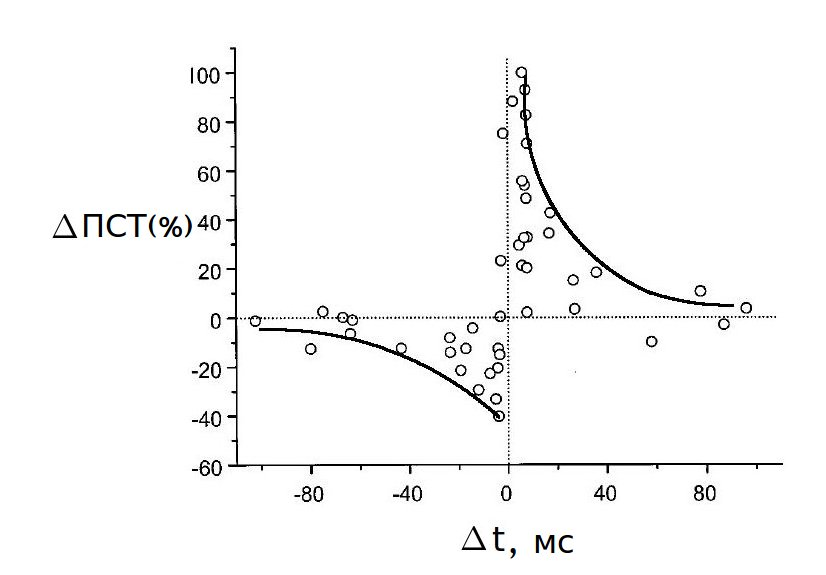
\includegraphics[width=75mm,scale=0.7]{stdp.jpg}
\caption{Спайко-временная пластичность. Зависимость $\Delta t = t_{post} - t_{pre}$ от изменения постсинаптического тока (ПСТ) на синапсе. Адаптировано из работы Г. Би и М. Пу \cite{stdp4}. }
\label{stdp_pic}
\end{figure}
\FloatBarrier
\indent Открытие этого феномена спровоцировало научное сообщество к новым дебатам на тему спайкового кода. С 1928-ого года, когда Э. Эдриан\cite{rate_first} предложил, что информация о стимуле хранится в спайковой активности усреднённой на относительно большом временном окне (100 мс), большинство нейрофизиологов на протяжении 20-ого века были на стороне данной гипотезы. В конце 20-ого века, мнения разделилсь, что послужило катализатором для новых исследований.\\
\indent Применение такого правила обучения в оригинальном виде можно реализовать непосредственным измерением $\Delta t = t_{post}-t_{pre}$ для $N$ пар пресинаптических и постсинаптических спайков
\begin{equation}\label{eq:sum_stdp}
\Delta w_{j} = \sum_{f=1}^N \sum_{n=1}^{N} W(t_{post}^{f} - t_{pre}^{n}),
\end{equation}
 и пропусканием через подобранную функцию $W(\Delta t)$, которая отражает зависимость на рис.\ref{stdp_pic}. Первое приближение такой зависимости наиболее удачно выражают две экспоненты
\begin{equation}
\begin{split}
W(x) &=\begin{cases} \, A_{+} exp(-x/\tau_{+}), & \mbox{если }x>0\mbox{,} \\ -A_{-} exp(-x/\tau_{-}), & \mbox{если }x<0\mbox{,} \end{cases}
\end{split}
\end{equation}
где $A_{+},A_{-},\tau_{+}, \tau_{-}$ константы, подобраные так, чтобы наилучшим образом приближать феноменологическую зависимость, их значения можно найти в оригинальной работе\cite{SongStdp}.\\
\indent Феноменологическая модель спайко-временной пластичности, по сути, основана на аппроксимации кривых полученных в экспериментах, как следствие имеет недостаток теоретической оправданности. Это правило обучение, являясь обучением без учителя, сложно интерпретировать и нельзя сказать точно какую статистику выражает нейрон обученный по этому правилу. Данный вопрос активно исследуется теоретиками нейронаук по всему миру.\\
\indent Однако, стоит заметить, что STDP играет роль и в контексте обучения с учителем. Группа F. Ponulak разработала правило обучения спайковых нейронных сетей ``ReSuMe''\cite{ponulak2010supervised}, в основе которого лежит STDP, модифицируемый фактором, который поощряет направление изменение синапсов по правилу STDP, если нейрон издал спайки близкие к целевым, и тормозит, в обратном случае.\\   
\subsubsection{Спайко-временная пластичность для триплета спайков}
\indent Работы описавшие спайко-временной пластичность были проделаны для низкочастотных повторений спайков и стоит отметить, что спайко-временная пластичность в том виде, как она представлена в работе Г. Би и М. Пу\cite{stdp4}, находится в противоречии со старыми работами в этой области, в которых долговременная депрессия и долговременная потенциация синапсов наблюдалась при стимуляции низкочастотными и высокочастотными спайками, соответственно\cite{caporale2008spike}, и, кроме этого, присутствует противоречие с исследованиями проведёнными БКМ теоретиками\cite{Cooper}. Более детально противоречия показали эксперименты\cite{bi2002temporal,froemke2002spike,wang2005coactivation} где спайко-временная пластичность в виде представленном на рис. \ref{stdp_pic}, не повторяет себя полностью для трёх и четырех спайков.\\
\indent В работе Pfister и Gerstner\cite{PfisterTriple} представлена модель спайко-временной пластичности, как попытка преодолеть все вышеназыванные противоречия.\\
\indent При приходе пресинаптического спайка на возбуждающий синапс во время $t_{pre}$, нейромедиатор высвобождается в синаптическую щель, где связывается с постсинаптическими рецепторами. Возьмём переменную $r_{1}$, которая будет отвечать за количество нейромедиатора на постсинаптической мембране. Во время пресинаптического спайка переменная увеличивается на $1$, после чего экспоненциально убывает со скоростью $\tau_{+}$
\begin{equation}
\frac{dr_{1}(t)}{dt} = -\frac{r_{1}(t)}{\tau_{+}}, \mbox{ если } t=t_{pre}\mbox{, то }r_{1} \rightarrow r_{1} + 1.
\end{equation}
\indent Основная идея Pfister и Gerstner заключается в том предположении, что существует ещё, как минимум, одна переменная $r_{2}$, которая ведёт себя аналогично переменной $r_{1}$, но на рабочем интервале $\tau_{x}>\tau_{+}$. Также вводятся переменные отражающие динамику постсинаптического нейрона $o_{1}$ и $o_{2}$, во времена спайков которого, переменные аналогично $r_{1}$ и $r_{2}$ увеличваются на $1$, с интервалами убывания $\tau_{-}$ и $\tau_{y}$, соответственно
\begin{equation*}
\frac{dr_{2}(t)}{dt} = -\frac{r_{2}(t)}{\tau_{x}}, \mbox{ если } t=t_{pre}\mbox{, то }r_{2} \rightarrow r_{2} + 1,
\end{equation*}
\begin{equation}
\frac{do_{1}(t)}{dt} = -\frac{o_{1}(t)}{\tau_{-}}, \mbox{ если } t=t_{post}\mbox{, то }o_{1} \rightarrow o_{1} + 1,
\end{equation}
\begin{equation*}
\frac{do_{2}(t)}{dt} = -\frac{o_{2}(t)}{\tau_{y}}, \mbox{ если } t=t_{post}\mbox{, то }o_{2} \rightarrow o_{2} + 1,
\end{equation*}
\indent Биологическая интерпретация переменных $r_{1}(t),r_{2}(t), o_{1}(t), o_{2}(t)$ может быть разной и кандиндатов на их роль много: пресинаптические переменные могут быть количеством нейромедиаторов в синаптической щели или количество активных НМДА рецепторов на постсинаптической мембране. На роль постсинаптических переменных может претендовать концентрация кальция на синапсе или обратное распространения потенциала на синапс во время постсинаптического спайка \\
\indent Изменение весов контексте данной модели производится при помощи выражений
\begin{equation}
\begin{split}
\Delta w &= - o_{1}(t)[A_{2}^{-}+A_{3}^{-}r_{2}(t-\boldsymbol{\epsilon})], \mbox{ если } t=t_{pre},\\
\Delta w &= r_{1}(t)[A_{2}^{+}+A_{3}^{-}o_{2}(t-\boldsymbol{\epsilon})], \mbox{ если } t=t_{post},
\end{split}
\end{equation}
где $A_{2}^{+},A_{2}^{-}$ - амплитуды потенциации и депрессии синапса, соответственно, в случае присутствия пар спайков на синапсе и нейроне, $A_{3}^{+},A_{3}^{-}$ - амплитуды потенциации и депрессии для случая триплета спайков. $\boldsymbol{\epsilon}$ - маленькая положительная константа, говорящая о том, что обновление весов должно происходить раньше обновления $r_{2}(t)$ и  $o_{2}(t)$.\\
\indent Это правило обучение ведёт себя аналогично обычной, парной спайко-временной пластичности при низкочастотных стимуляциях (1 Гц). При высоких частотах спайковых стимуляций правило показало лучшее соответствие экспериментальным данным, даже в случае сложных паттернов спайков.\\
\indent Отдельно стоит выделить, что Pfister и Gerstner проделали выкладки и симуляции доказывающие, что в случае усреднения спайковых паттернов на нейроне и синапсе, правило ведёт себя аналогично правилу из БКМ теории.\\


\subsubsection{Теоретическая оптимальная модель спайко-временной пластичности}
\indent Одна из попыток теоретизировать спайко-временную пластичность являтся серия работ T.Toyoizumi и др.\cite{OptStdpFirst, OptStdpSecond}. В основу этой модели заложена гипотеза, что динамика синапсов происходит таким образом, что активность нейрона становится более информационно насыщенной по Шеннону.\\
\indent В случае одного нейрона и $N$ синапсов, входной сигнал можно представить в виде набора пресинаптических спайков $X(T)=\{ x_{j}(t)=\sum_{t_{j}^f}\delta(t-t_{j}^f) |j=1,...,N, 0 \leq t<T \}$, и выходной сигнал в виде спайков нейрона $Y(T)=\{ y_{j}(t)=\sum_{t_{post}^f}\delta(t-t_{post}^f) | 0 \leq t<T \}$, где $T$ время эксперимента, $\delta(t)$ - дельта функция имеющая значение $1$ в нуле, и $0$ в любой другой области. Информацию, которую передаёт нейрон, как стохастичный элемент, можно записать 
\begin{equation}\label{eq:opt_stdp_I}
I = \la\log \frac{P(Y|X)}{P(Y)} \ra_{Y,X},
\end{equation}
где $P(Y|X)$ условная плотность вероятности сгенерировать нейроном конкретный набор спайков $Y$ на протяжении времени $T$ при данном входном наборе спайков синапсов $X$, $P(Y)$ - плотность вероятности сгенерировать набор спайков $Y$ не зная вход $X$.\\
\indent Основаная гипотеза T.Toyoizumi заключается в том, что динамика синапсов нейрона направлена на то, чтобы максимизировать выражение \eqref{eq:opt_stdp_I}. Чтобы привести эту задачу к задаче оптимизации достаточно выразить плотности вероятностей и взять производную по параметру весов синапсов, чтобы можно было осуществить градиентный подъем по информации выходного сигнала нейрона.\\
\indent Выражение плотностей вероятности генерации спайков в выражении \eqref{eq:opt_stdp_I} зависит от выбранной модели спайкового нейрона. В случае модели Spike Response Model из раздела \ref{sec:srm}, выбрав функцию активации $p(t)$, выразить плотности не составляет труда
\begin{equation}\label{eq:opt_stdp_pyx}
P(Y|X)= \prod_{t_{post}^{f} \in Y } p(t_{post}^{f}) \int_{0}^{T} exp(-p(t))dt\;,
\end{equation}
причем $P(Y)$ можно вывести аналогично \eqref{eq:opt_stdp_pyx}, но для усреднённой плотности вероятности по всем $X$: $\bar{p}(t) = \langle p(t) \rangle _{X}$.\\
\indent Производную выражения \eqref{eq:opt_stdp_I} по параметру $w_{j}$, где $w_{j}$ вес синапса $j$ SRM модели, можно записать
\begin{equation}\label{eq:opt_stdp_Idw}
\frac{dI}{dw_j} = \la \frac{1}{P(Y|X)}\frac{dP(Y|X)}{dw_{j}}\log\frac{P(Y|X)}{P(Y)} \ra_{Y,X}
\end{equation} 
взяв выражение потенциала мембраны SRM модели $u(t)$ \eqref{eq:srm} вместе с любой, интегрируемой на всей области, функции активации $p(u)$, можем записать второй множитель из уравнения \eqref{eq:opt_stdp_Idw} таким образом
\begin{equation}\label{eq:opt_stdp_dp_dw}
\frac{dP(Y|X)}{dw_{j}} = P(Y|X)\int_{0}^{T} c_{j}(t)dt,
\end{equation} 
где
\begin{equation}
c_{j}(t) = \frac{p'_{u}(t)}{p(t)}[y(t)-p(t)]\int_{0}^{\infty}ds'\epsilon(s') x_{j}(t-s'),
\end{equation} 
а также третий множитель 
\begin{equation}
\log\frac{P(Y|X)}{P(Y)} = \int_{0}^{T}B^{post}(t)dt,
\end{equation}
где
\begin{equation}
B^{post}(t) = y(t)\log \frac{p(t)}{\bar{p}(t)} - (p(t)-\bar{p}(t)),
\end{equation} 
первый множитель при подстановке \eqref{eq:opt_stdp_dp_dw} в \eqref{eq:opt_stdp_Idw} сокращается.\\
\indent Таким образом, совокупив выкладки выше, можно записать\\
\begin{equation}\label{eq:opt_stdp_Idw_final}
\frac{dI(t)}{dw_j} = \int_{0}^{T} dt \int_{0}^{T} c_{j}(t')dt' B_{post}(t) \rangle _{X,Y}.
\end{equation}
\indent Второй интеграл выражения \eqref{eq:opt_stdp_Idw_final} вместо изнурительных подсчётов удобно усреднять на временном промежутке $\tau_{C}$ 
\begin{equation}
\frac{dC(t)}{dt} = c_{j}(t) + \frac{C(t)}{\tau_{C}},
\end{equation}
при условии, что $\tau_{C}$ больше чем масштаб автокорелляционной функции активности нейрона.\\
\indent В итоге, как следствие всех выкладок, можно получить динамику веса во времени
\begin{equation}\label{eq:opt_stdp_dw_dt}
\frac{dw_{j}(t)}{dt} = \alpha[C_{j}(t)B^{post}_{i}(t)]
\end{equation}
где $\alpha$ -- маленький коэффциент обучения.\\
\indent Переменные $c_{j}(t)$ и $B_{post}$ несут в себе свою смысловую нагрузку. Переменная $c_{j}(t)$ характеризуется входящими в неё произведением пресинаптической и постсинаптической активности, $x_{j}(t)$ и $y(t)$ соответственно. Таким образом, $c_{j}(t)$ является корреляцией активностей синапса $j$ и нейрона, и сильно напоминает Хэббо-подобные правила обучения для усреднённых активностей. Как упоминалось в разделе \ref{sec:hebb}, в чистом виде, правило Хэбба ведёт к нестабильному росту весов и переменная $B_{post}(t)$ в \eqref{eq:opt_stdp_dw_dt} ведёт себя как фактор, который привносит в обучение интеллектуальность -- происходит поощрение только тех активностей, которые отличаются от средней и имеют информационную значимость\cite{OptStdpFirst}.\\
\indent Таким образом, максимизируя только информацию, которую передаёт нейрон, правило обучения возвращает нас к правилу правилу Хэбба с модификацией. Больше того, в первой работе\cite{OptStdpFirst}, произведены выкладки и эксперименты, которые позволяют сравнить это правило обучения с динамикой БКМ правила, что вселяет надежды, найти универсальное, биологически и теоретически оправданное, правило обучения нейронных сетей.

\section{Применения спайковых нейронных сетей}
\indent Кроме таких частных фирм как, например, Spikenet Technology, Brain Corporation широкое промышленное применение спайковые нейронные сети не нашли и только в начале своего пути. Однако, тема спайковых нейронных сетей активно развивается группами учёных по всем миру, и, на сегодняшний день, огромное количество исследований производится по данной тематике.
\subsection{Распознавание образов}
\indent В работах группы Thorpe\cite{thorpe2001spike,guyonneau2004temporal,perrinet2004sparse} был предложен метод для быстрого распознавания образов используя STDP обучение (\ref{sec:stdp}) и т.н. кодирование порядком спайков (rank-order coding). Архитектура сети состояла из двух слоёв нейронов. На каждый шаг обучения, одна из картинок для классификации была представлена сети, что вызывало по одному спайку от каждого нейрона в первом слое, причем время спайка зависит от интенсивности области, за который отвечает нейрон первого слоя -- чем сильнее интенсивность, тем раньше будет произведен спайк. Первый спайк, который издал нейрон второго слоя, тормозил активность других нейронов при помощи латеральных связей и вызывал STDP обучение. Как результат обучения на пуле картинок для категоризации, нейроны второго слоя сформировали чувствительность к определённым, наиболее частостным признакам, что позволило построить классификатор на базе этой архитектуры.\\
\indent Также, используя фрейморк предложенный Thorpe, в работе\cite{kornprobst2005could} была построена спайковая нейронная сеть для распознования динамических образов из видеоряда. В работе\cite{shin2010recognition} предложена иерархическая спайковая нейронная сеть на основе Integrate-and-fire нейронов, для классификации частично обозримых и повернутых изображений.\\
\indent Распознование лиц в движении было произведено в работе Wysoski\cite{wysoski2008fast} используя динамическое формирование структуры сети и Хэббо-подобное правило обучение.
\subsection{Задачи управления, контроля и принятия решений}
\indent В работе Ponulak\cite{ponulak2006resume} предложена архитектура спайковой сети для решения задачи управления роботом при помощи правила обучения ``ReSuMe''. Также в работах D. Paolo \cite{paolo2003a, paolo2003b} рассмотрен эволюционный подход к обучению спайковой нейронной сети со спайко-временной пластичностью. Робот должен был воспроизвести положительный фотоаксис (движение к источнику света) в случае отсутствия звукого стимула и отрицательный фотоаксис в случае присутствия неприятного короткого звукового сигнала. Были рассмотрена нейронные сети двух видов: классические ИНС с усреднённой активностью и спайковые ИНС. Показано, что в одинаковых условиях, спайковый контроллер находит стабильное состояние быстрее и надежнее чем сети с усреднённой активностью. Также, эволюционный подход и спайковый нейронные сети показали себя в решении задачи управления мобильным роботом в работе\cite{trhan2012application}.\\
\indent Для задачи принятия решений в работе\cite{glackin2008implementing}, была предложена спайковая нейронная сеть, которая обучалась Хэббо-подобным правилом обучения с учителем. 
\subsection{Классификация временных данных}
\indent Спайковые нейронные сети, также, показали себя, как классификаторы временных сигналов в таких задачах как классификация спайковых паттернов\cite{ponulak2010supervised,maass2002paradigms}, распознавание речи\cite{brody2003simple,gutig2009time} и классификации электроэнцефалограмм для случаев эпилептичных припадков\cite{ghosh2009new}.\\
\indent Хотя без использования ИНС, но достойна внимания работа\cite{smith2006efficient}, в которой представлен алгоритм оптимальной репрезентации звуковых сигналов в виде спайковых паттернов. Применение биологически оправданных кохлеарных фильтров, показало, что именно спайковое представление является наиболее оптимальным для последующей классификации или восстановления сигнала.\\
\indent Показано применение кодирования порядком спайков для распознования речи в работе Loiselle и др.\cite{loiselle2005exploration}. Для небольшого набора данных спайковая нейронная сеть показала себя лучше чем скрытая марковская модель, однако, это сеть не показала себя лучше для б\'{о}льшей выборки.\\
\indent В работе Wang и Pavel\cite{wang2005spiking} рассмотрена спайковая нейронная сеть, которая основываясь на свойствах рефракторности нейронов представляла сигнал в виде спайкового кода. Амплитуда сигнала конвертировалась в спайк определенного временного порядка, и сигнал представлялся в виде межспайковых интервалов.\\
\section{Выводы}
\indent Не смотря на то, что спайковые нейронные сети только в начале своего пути и пока нельзя сказать об их  полномасштабном промышленном использовании, это остаётся перспективной и интересной областью развития вычислительной нейронауки.\\
\indent Характерным отличием спайковых нейронных сетей от классических, является наличие внутреннего состояния, которое характерно для большинства более менее сложных динамических процессов. Наличие внутреннего состояния делает спайковые сети естесственными для обработки временных данных и задач аппроксимации контроля динамическими системами.\\
\indent Стоит отметить некую дуальность, которую в себе несёт исследование спайковых нейронных сетей: во-первых, это поиск новых нейронных моделей, которые могут быть лучше старых для конкретных задач, во-вторых это исследование биологических нейронных сетей и нюнсов информационной обработки так, как это делает настоящий биологический нейрон.\\

\bibliography{refs}{}
\bibliographystyle{unsrt}

\end{document}
